%%%%%%%%%%%%%%%%%%%%%%%%%%%%%%%%%%%%%%%%%
% Uppsala University Assignment Title Page 
% LaTeX Template
% Version 1.0 (27/12/12)
%
% This template has been downloaded from:
% http://www.LaTeXTemplates.com
%
% Original author:
% WikiBooks (http://en.wikibooks.org/wiki/LaTeX/Title_Creation)
% Modified by Elsa Slattegard to fit Uppsala University
% License:
% CC BY-NC-SA 3.0 (http://creativecommons.org/licenses/by-nc-sa/3.0/)
%TC:incbib
%\title{Title page with logo}
%----------------------------------------------------------------------------------------
%	PACKAGES AND OTHER DOCUMENT CONFIGURATIONS
%----------------------------------------------------------------------------------------

\documentclass[12pt]{article}
\usepackage[english]{babel}
\usepackage[utf8]{inputenc}
\usepackage{amsmath}
\usepackage{graphicx}
\usepackage{microtype}
\usepackage[font=small,labelfont=bf]{caption}
\setlength{\parindent}{0pt}
\setlength{\parskip}{0.25em}
\setlength{\textfloatsep}{10pt plus 2pt minus 2pt}
\setlength{\intextsep}{8pt plus 2pt minus 2pt}
\usepackage{float}
\usepackage[nottoc,numbib]{tocbibind}
\setlength{\marginparwidth}{2cm}
\usepackage[colorinlistoftodos]{todonotes}
\usepackage{hyperref}
\hypersetup{hidelinks}

\begin{document}

\begin{titlepage}

\newcommand{\HRule}{\rule{\linewidth}{0.5mm}} % Defines a new command for the horizontal lines, change thickness here
\center % Center everything on the page
 
%----------------------------------------------------------------------------------------
%	HEADING SECTIONS
%----------------------------------------------------------------------------------------

\textsc{\LARGE Uppsala University}\\[1.5cm] % Name of your university/college
\IfFileExists{Uppsala_University_seal_svg.png}{\includegraphics[scale=.1]{Uppsala_University_seal_svg.png}}{}\\[1cm] % University logo is optional; add the file to this folder if available

%----------------------------------------------------------------------------------------
%	TITLE SECTION
%----------------------------------------------------------------------------------------

\HRule \\[0.4cm]
{ \huge \bfseries Assistive Driving System}\\[0.4cm] % Title of your document
\HRule \\[1.5cm]
 
%----------------------------------------------------------------------------------------
%	AUTHOR SECTION
%----------------------------------------------------------------------------------------

\begin{minipage}{0.6\textwidth}
\begin{flushleft} \large
\emph{Authors:}\\
Sami Al Saati\newline
Murithado Abdulrazaq\newline
Issac Samuel Paul\newline
Jinjie Tang\newline
Aravinda Prasad Arumugam\\
\end{flushleft}

\end{minipage}\\[2cm]

% If you don't want a supervisor, uncomment the two lines below and remove the section above
%\Large \emph{Author:}\\
%John \textsc{Smith}\\[3cm] % Your name

%----------------------------------------------------------------------------------------
%	DATE SECTION
%----------------------------------------------------------------------------------------

{\large \today}\\[2cm] % Date, change the \today to a set date if you want to be precise
\vfill % Fill the rest of the page with whitespace

\end{titlepage}

\thispagestyle{empty} % No page number on title page
\newpage
\tableofcontents
\clearpage
\section{Introduction}

We will build an assistive driving system on a Raspberry Pi, using sensors that detect objects close to the car. It warns the driver when reversing and when something is in a blind spot, and it is meant to be installed on a car.

Some drivers have reduced vision, whether because of age or other reasons, while still meeting the legal requirements to drive. This may make it harder to judge distances and notice objects around the car, for example when reversing or changing lanes. Parking sensors and blind spot warnings can help in these situations, but they are usually found in newer or more expensive cars. Drivers with older cars may therefore not have access to them. Our product aims to give these drivers extra awareness, which could make driving less stressful and may lower the risk of collisions.

Our project focuses on equity and accessibility. Access to these safety features currently depends on which car a person can afford. By developing a cheap aftermarket add-on, we hope to make this kind of safety feature available to more people who could benefit from it, regardless of their budget or the age of their car. 
\subsection{Use cases}
\subsubsection{Reversing}
When backing out of a parking space or a driveway, a pillar, parked car, or a child behind the car can be hard to see. Our system serves to measure the distance to objects behind the car and beeps faster as the car gets closer to the person or object.

\subsubsection{Chaning lanes}
The same driver may have trouble checking the blind spot of the car. Our system detects objects in the blind spot and warns the driver before they change lanes.
\clearpage
\section{Related works}
The use of ultrasonic sensors are widely explored in short range obstacle detection systems because of their practicality and low computation requirements; not requiring many resources due to the absence of image processing. In the paper by Agarwal et al. \cite{agarwal2009cost} they developed a low cost ultrasonic driver assistance system for close range obstacle detection, also ensuring the reduction of crosstalk between multiple sensors to reduce misinterpretations and false positives. Similarly, Alonso et al. \cite{alonso2011ultasonic} investigated the use of ultrasonic sensors, but in the context of urban traffic and evaluated it in real traffic conditions. These studies provide a foundation of the design goal, focusing on short range obstacle detection with low cost resources.

Research in obstacle detection also emphasizes the importance of sensor placement and environmental perception. Wu et al. \cite{wu2019implementation} viewed the feasibility of using ultrasonic sensors in the context of automated parking, using the distance measurements to optimise and guide parking manoeuvres. Eisele et al. \cite{eisele2024relevance} illustrated that using object distance detection to classify objects based on the echoes is not viable as they are separate challenges. Our prototype, to reduce the complexity and focus on affordability does not include object classification and solely relies on distance detection.

Effective communication of obstacle information to users is a crucial consideration in the design of assistive technologies and the following articles encapsulate this. Dos Santos et al. \cite{dos2021systematic} reviewed wearable devices that support mobility and orientation among people with visual impairments and highlighted the importance of audio feedback. They also emphasize proper safety testing and the need of the participation of users in the prototype evaluation. Xu et al. \cite{xu2023wearable} similarly reviewed and highlighted the importance of considering safety and utility of the technology for the users. Hersh argues that technical performance should be complemented by practical usability in everyday environments \cite{hersh2022wearable}.

Several other individual studies demonstrate how these technologies can be implemented. Froneman et al. \cite{froneman2017development} explored the idea of a wearable device equipped with ultrasonic sensors and vibration feedback to assist visually impaired users. Jubril and Samuel combined ultrasonic sensing, camera and laser based techniques to detect obstacles, their system especially handles detecting smaller holes and obstacles that may exist in the users path \cite{jubril2021multisensor}. Xu et al. \cite{xu2023wearable} reviewed wearable obstacle-avoidance electronic travel aids for blind and visually impaired individuals, highlighting approaches to assistive obstacle detection. These approaches demonstrate the value of providing intelligible feedback, although the domain of pedestrian navigation differs significantly from vehicle navigation.

Our project differs in that we prioritise simplicity and affordability, utilising a rear sensor to support reversing and a side sensor to detect objects in blind spots.

\clearpage
\section{Methods and tools}
The implementation leverages a modular, decoupled architecture consisting of an embedded control layer and a real-time remote telemetry interface:

\begin{itemize}
    \item \textbf{Operating System:} Raspberry Pi OS (Lite, 64-bit). A minimal, headless Linux distribution is selected to reduce background process overhead, minimize latency, and preserve CPU cycles for deterministic sensor polling and motor control loops.
    \item \textbf{Primary Programming Language:} Python 3. Python provides rapid prototyping capabilities and extensive library ecosystems for embedded hardware interfacing and asynchronous network communication.
    \item \textbf{Hardware \& GPIO Libraries:}
    \begin{itemize}
        \item \texttt{gpiozero} / \texttt{RPi.GPIO}: High-level abstractions for reading ultrasonic trigger/echo timings, driving digital logic lines on the H-bridge, and toggling alerts.
        \item \texttt{pigpio}: Utilized for direct access to the Broadcom hardware timers, generating jitter-free Hardware Pulse Width Modulation (PWM) signals for the steering servo and passive buzzer.
    \end{itemize}
 
    \item \textbf{Development \& Tooling:} Git for version control, VS Code with Remote-SSH extension for on-target development, and \LaTeX{} for technical documentation and specification reporting.
\end{itemize}

\clearpage
\section{Potential Obstacles and Mitigation Strategies}

\begin{enumerate}
    \item \textbf{Non-Real-Time Linux OS Latency and Timing Jitter:}
    \begin{itemize}
        \item \textit{Obstacle:} Standard Linux is not a hard Real-Time Operating System (RTOS). Kernel thread scheduling and context switching can disrupt microsecond-level timing measurements required by the HC-SR04 ultrasonic echo pulses, resulting in false distance spikes.
        \item \textit{Mitigation:} Distance measurement routines will implement rolling median filters and threshold clamping to reject spurious outlier readings. Critical PWM signals (servo angle and buzzer pitch) will be mapped strictly to hardware-timed PWM channels (GPIO 12, 13, 18, or 19) rather than software-emulated PWM loops.
    \end{itemize}

    \item \textbf{Ultrasonic Acoustic Limitations and Blind Spots:}
    \begin{itemize}
        \item \textit{Obstacle:} HC-SR04 sensors have a narrow operational beam angle ($\approx 15^\circ$) and rely on specular acoustic reflection. Angled surfaces, acoustic-absorbent fabrics, or obstacles outside the direct line of sight can cause sound waves to deflect away, resulting in missed detections.
        \item \textit{Mitigation:} Sensor thresholds will incorporate a safety buffer zone ($<15$\,cm emergency stop), and the chassis will mount sensors at optimal bumper height. Software interlocks will treat timeout errors (lost echo pulses) as potential obstructions by defaulting to a safe, reduced-speed state.
    \end{itemize}

    \item \textbf{Voltage Level Incompatibility (5V vs. 3.3V Logic):}
    \begin{itemize}
        \item \textit{Obstacle:} The HC-SR04 operates at 5\,V $V_{CC}$ and returns a 5\,V TTL logic HIGH on the \texttt{Echo} pin. Direct connection to the Raspberry Pi GPIO header will cause electrical overstress and permanently destroy the Broadcom SoC pins, which are strictly 3.3\,V tolerant.
        \item \textit{Mitigation:} A dedicated passive voltage divider network (composed of a 1\,k$\Omega$ series resistor and a 2\,k$\Omega$ pull-down resistor) will step down the 5\,V echo return to a safe $\approx 3.33$\,V reference before reaching the GPIO input.
    \end{itemize}

\end{enumerate}

\clearpage
\section{Ethical considerations}
\subsection{Safety and Reliability}
Safety and Reliability are the main ethical considerations for this project. The product is designed to assist drivers by detecting obstacles around the car. Inaccurate sensor readings and missed detections will result in tragic accidents, which may cause life-threatening dangers to users. Therefore, the product should be tested rigorously to evaluate its detection accuracy and limitations. And developers should state clearly that this device is just an additional assistance, which cannot completely replace the driver's accountability to drive the vehicle safely.

\subsection{Equity and Accessibility}
The goal of this project is to achieve equity and accessibility, making safety affordable for drivers who do not have newer vehicle models. However, accessibility does not merely include affordability. The device should also be easy to install and compatible with distinct vehicle models.

\clearpage
\section{Implementation}
The system runs on a Raspberry Pi 3 Model B with Raspberry Pi OS (64-bit). It is configured for headless operation and developed remotely over SSH. HC-SR04 ultrasonic sensors measure distance, with one intended to face backwards for reversing and another on the side for blind-spot detection. A buzzer provides audible alerts. Each Echo line passes through a voltage divider to protect the Raspberry Pi's 3.3 V GPIO pins, and a power bank supplies power independently of the car.

The software reads sensor measurements, smooths the results with a rolling median filter to reduce isolated fluctuations, and maps the measured distance to an alert level. In the integrated prototype, the buzzer is controlled through PWM: danger produces a continuous tone, warning produces faster intermittent beeps, and caution produces slower intermittent beeps. The web dashboard displays the measured distance, obstacle classification, sensor status, and buzzer state. The application is configured to start automatically at boot through a \texttt{systemd} service. The source code is available at \url{https://github.com/aravindvinas/Assistive-Driving-System.}

\begin{figure}[htbp]
    \centering
    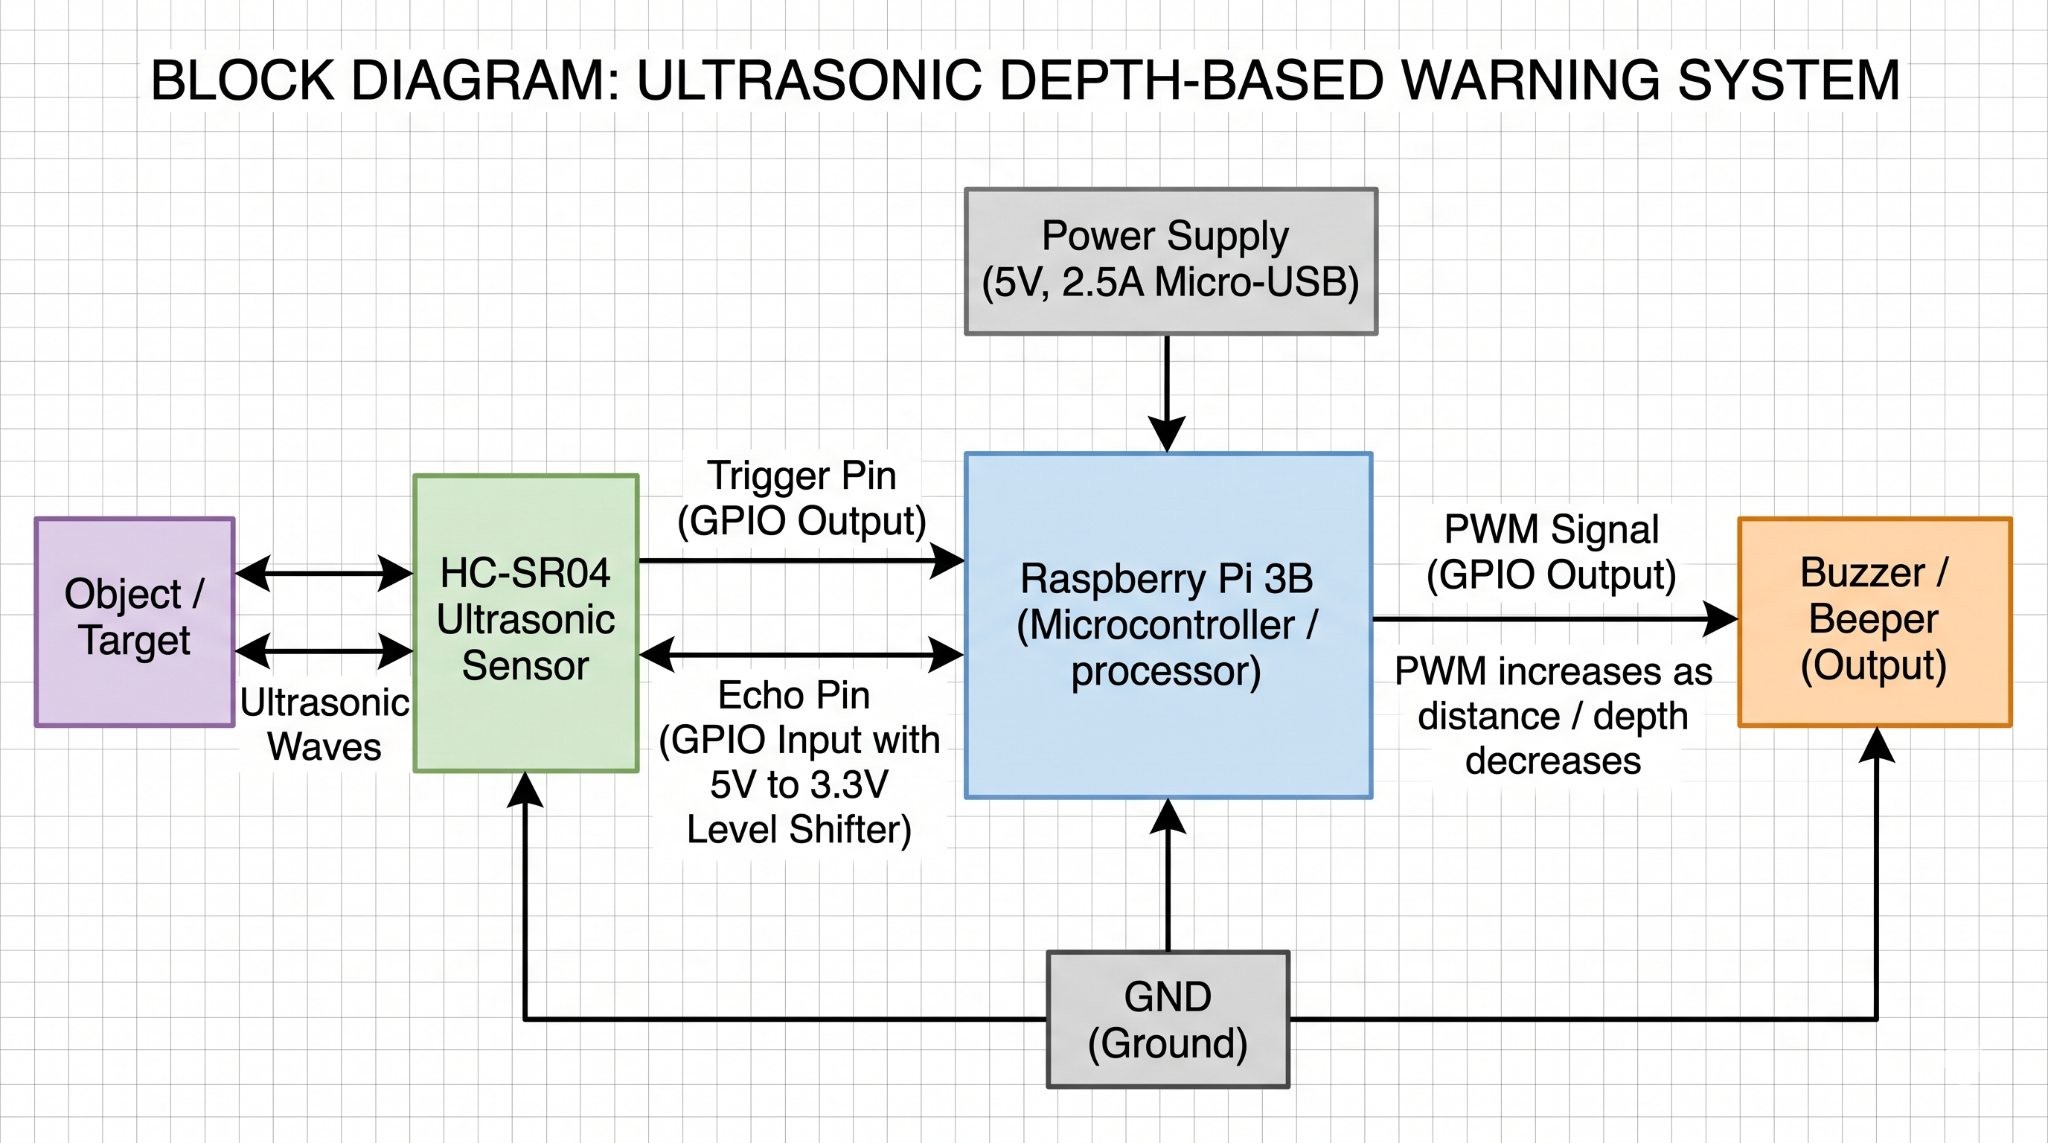
\includegraphics[width=0.98\linewidth,height=0.48\textheight,keepaspectratio]{Assistive_Driving_Block_Diagram.png}
    \caption{Block diagram of the ultrasonic depth-based warning system.}
    \label{fig:assistive-driving-block-diagram}
\end{figure}

\clearpage
\section{Results and Discussion}

\subsection{Test Setup}

The prototype was tested on a bench using a Raspberry Pi 3 Model B, an HC-SR04 ultrasonic sensor, a PWM-controlled buzzer, and a phone-accessible web dashboard. The application runs as a \texttt{systemd} service. Testing focused on sensor readings, distance classification, dashboard updates, and service operation after startup.

\subsection{Distance Measurement}

The sensor produced readings of approximately 308--310\,cm when no nearby obstacle was detected. When an object was brought closer, earlier tests recorded readings of approximately 17--22\,cm. The logs show that raw measurements and smoothed values were reported repeatedly, demonstrating continuous polling. A rolling median filter was used to reduce short-lived fluctuations, although smoothing can delay the displayed response when distance changes quickly.

\subsection{Obstacle Classification and Audible Alerts}

The software uses four distance zones: safe (above 100\,cm), caution (above 60\,cm and up to 100\,cm), warning (above 30\,cm and up to 60\,cm), and danger (30\,cm or less). The buzzer is configured for slower intermittent beeps in caution, faster beeps in warning, and a continuous tone in danger; it remains silent in safe and unknown states. The captured dashboard shows a safe reading and the buzzer off. Separate controlled tests at each threshold are still needed to document the accuracy of every alert transition.

\subsection{Web Dashboard}

The dashboard provides a live view of obstacle status, measured distance, buzzer state, sensor status, and the latest update time. As shown in Figure~\ref{fig:driving-dashboard}, the captured interface displayed \textit{SAFE}, a distance of 308.6\,cm, sensor status \textit{OK}, buzzer state \textit{OFF}, and Pi service status \textit{Online}. This confirms that the dashboard was accessible and receiving status data during the recorded test. The interface refreshes automatically, allowing a phone connected to the same local network to monitor the prototype.

\begin{figure}[htbp]
    \centering
    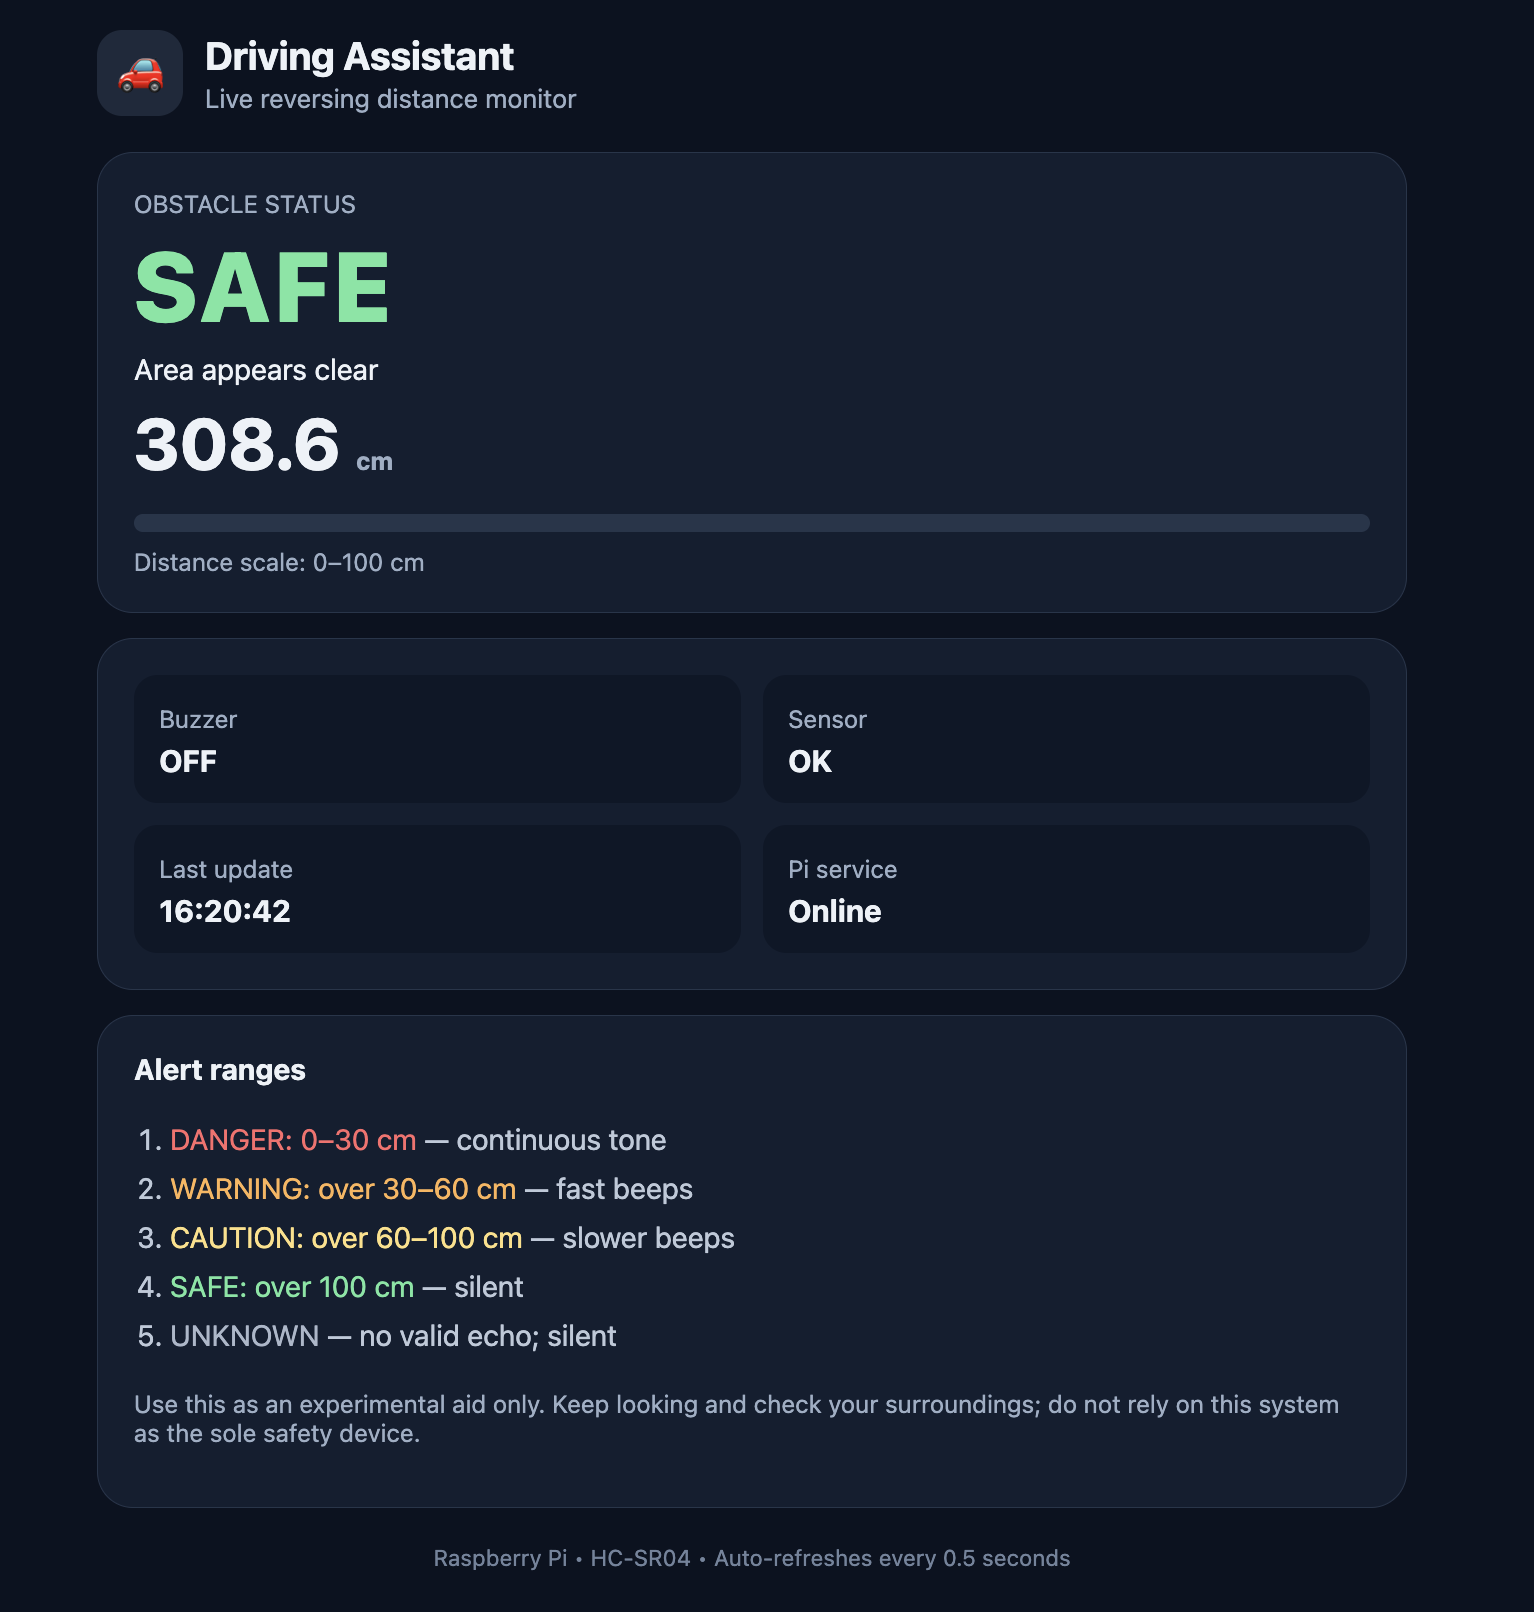
\includegraphics[width=0.78\linewidth,height=0.58\textheight,keepaspectratio]{Driving_Assistant_Dashboard.png}
    \caption{Live driving-assistant dashboard showing a safe distance reading and online service status.}
    \label{fig:driving-dashboard}
\end{figure}

\subsection{Automatic Startup and Service Logs}

The integrated application is managed by the \texttt{driving-assistant-allinone.service} systemd unit. The captured terminal output in Figure~\ref{fig:driving-service-log} shows that the service is loaded and enabled, its state is \textit{active (running)}, and the Python process is continuously logging raw and smoothed distance readings. The service was also tested through multiple power cycles, and the process continued to work after rebooting. These observations support that automatic startup and ongoing sensor polling were functioning during the recorded tests.

\begin{figure}[htbp]
    \centering
    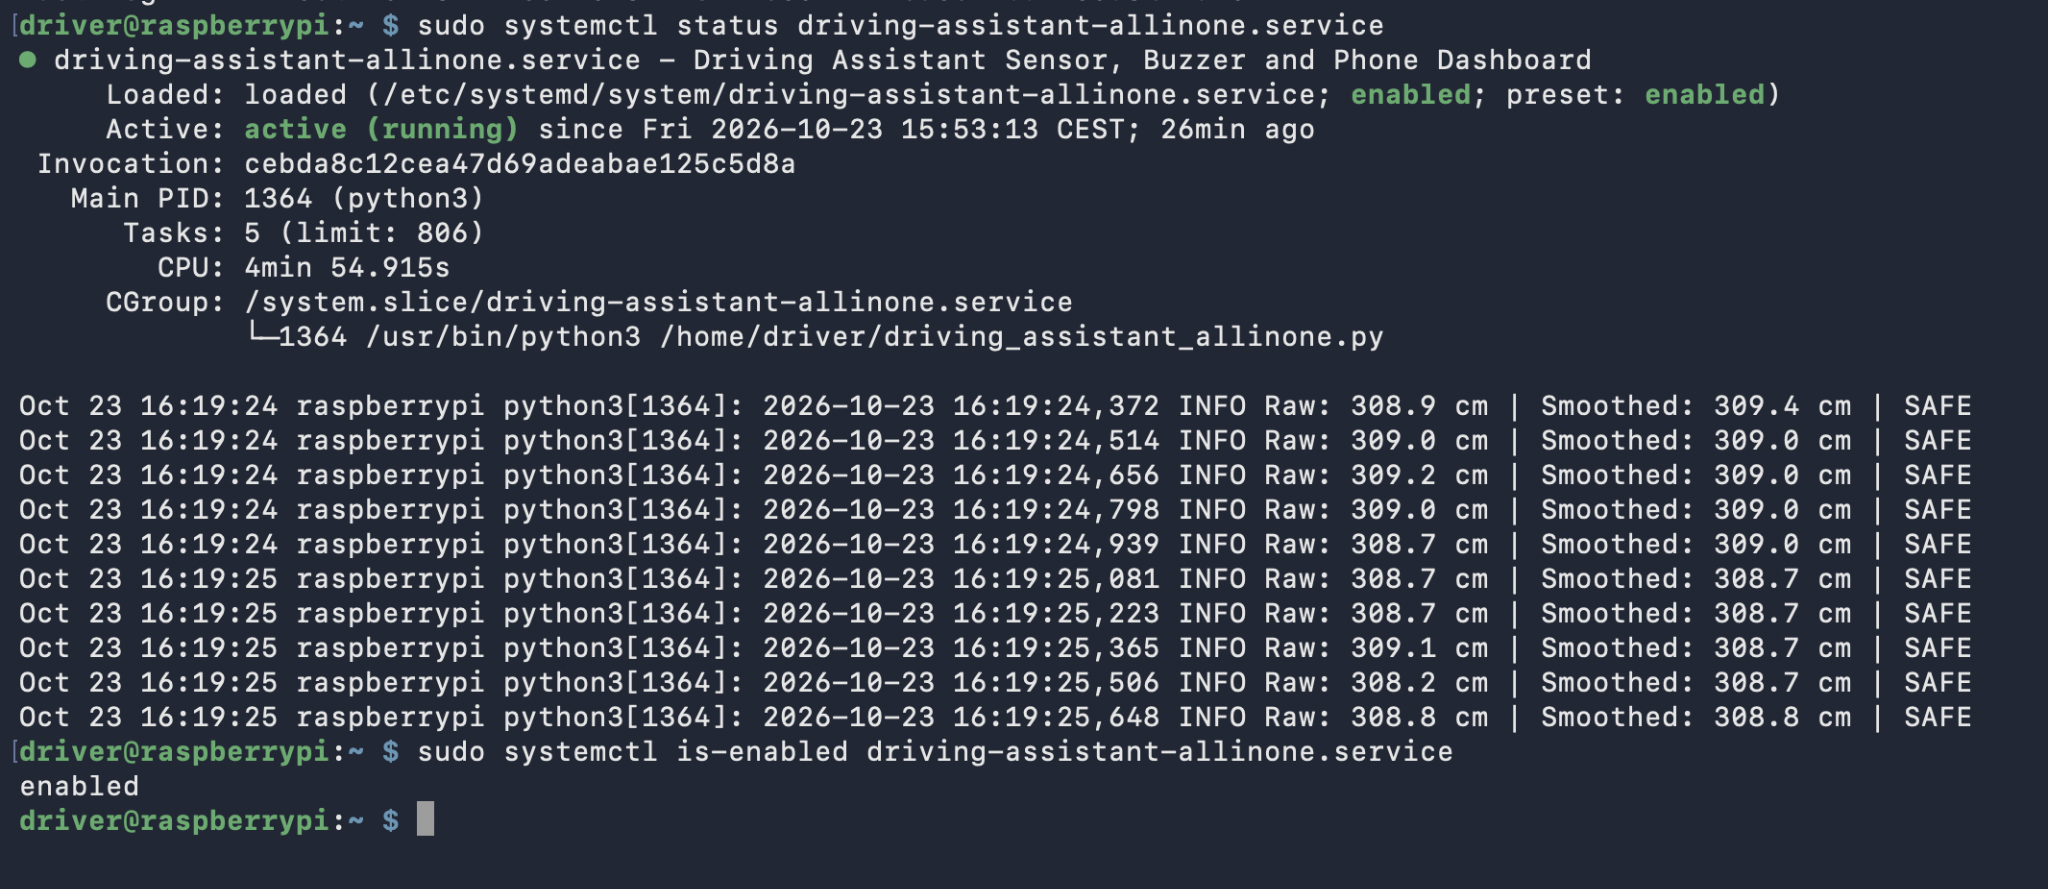
\includegraphics[width=0.98\linewidth,height=0.38\textheight,keepaspectratio]{Driving_Assistant_Service_Log.png}
    \caption{Systemd status and sensor logs showing the driving-assistant service running and enabled.}
    \label{fig:driving-service-log}
\end{figure}

\subsection{Discussion and Limitations}

The results demonstrate basic short-range obstacle detection, distance classification, a working live dashboard, and an enabled background service. The measured distance changes as an object approaches, while the dashboard and logs provide complementary visual and diagnostic feedback. Remaining limitations include ultrasonic sensitivity to target angle and surface, possible delay from smoothing, and the need to validate buzzer patterns at each threshold under repeatable conditions. Further work should measure accuracy at known distances, record alert response times, and test network reconnection on different hotspots. The prototype has been evaluated on a bench rather than in a vehicle and is not a certified safety system; it must not replace direct observation or established vehicle safety mechanisms.

\clearpage
\section{Conclusion and future work}
We have designed an assistive driving system using a Raspberry Pi 3 and HC-SR04 ultrasonic sensors, with the goal of helping drivers with reduced vision, for example due to age. A sensor in the rear helps when reversing, and a side sensor watches the cars blind spot. A buzzer warns the driver and beeps faster as the car gets closer to an object. The build consists of cheap parts that are easily found, which increases the accessibility. This gives drivers of older cars features that are usually only found in newer cars. We succeeded in providing a device acting as a proof of concept of what could be further developed. The system however needs some more development.

\newline
\newline
The next step is testing using a real car, in rain and with obstacles that the sensor may struggle to detect. Letting drivers from the target group use the system in everyday driving would also be helpful. Ultrasonic sensors have some limitations that need to be tested \cite{ept2021limitations}. A pedestrian in a winter jacket may be harder to detect, since fabric absorbs some of the signal. A thin pole may also be missed, because there is a smaller surface for the signal to bounce back from. The device should also be tested in different seasons, as the temperature can affect the signal, so a sensor that works in summer may not give the same readings in the winter. 

A potential improvement on the system could be to add a light that turns on if an object is detected, further decreasing the risk of collision.

A study could also check whether the system reduces the number of accidents.

\clearpage
\section{Scrum experience}
Our team used the Agile method throughout the project, following the Scrum framework to organize our work, track progress visibly, and ensure honest check-ins from each member. We organized and tracked our tasks using a Trello board, categorizing them into three stages: To Do, Doing, and Done. To share updates on tasks in a timely manner, we held daily standups on WhatsApp. Every other day, the facilitator conducted a Zoom meeting in which we discussed the progress in more detail and tried to come up with solutions to tackle the obstacles we faced in the project. We also met with our supervisor in person each week to review our progress and receive feedback on our completed work. Moreover, every Friday, each member is obligated to fill out the retrospective time log, which helps us reflect on our individual contributions and guarantee a fair distribution of workload across the team.

Overall, our team’s experience with Scrum was positive. It supported our teamwork in a more structured and collaborative way. Through the Trello board, we were able to monitor our progress and confirm that everybody clearly knows their responsibilities. The daily standups aided us in staying connected and informed, and the Zoom meeting provided opportunities to discuss hurdles and find out remedies together. With supervision, the sprint can stay on the right track, and the project can be enhanced through valuable feedback. The retrospective time logs help us to evaluate individual workload and avoid internal team conflict caused by unfairness. Even though Scrum is instrumental, we sometimes still face difficulties in coordinating schedules and finishing tasks within the planned time. However, over time, we became more flexible in our approach and learned to handle unexpected challenges more efficiently.

\newpage

\bibliographystyle{plain}
\bibliography{references}

\end{document}